%%%%%%%%%%%%%%%%%%%%%%%
%%      Lecon 5      %%
%%%%%%%%%%%%%%%%%%%%%%%

\chapter{Les leçons de la grande crise de 1929 :
similitudes et différences}

Avant de passer à la crise de 1929, on peut résumer les derniers cours dans leurs grandes lignes de la sorte : 

\begin{center}
	Innovation financière + exhubérance irrationnelle $\rightarrow$ faillite de grandes banques + perte de confiance (actionnaires, épargnants, etc.) $\rightarrow$ les Etats interviennent $\rightarrow$ économie réelle en difficulté $\rightarrow$ Etats endettés $\rightarrow$ entraîne l'Euro dans la tourmante.
\end{center} 

\section{Les crises dans l'histoire}
\subsection{Japon 1990}
Vers la fin des années '80, la bourse japonaise explose. La valeur des actions est haute et les taux d'intérêt sont assez bas (2.5\%). Cependant, en 1990, la première guerre du golf éclate. Ca entraine une chute de la demande (crise du pétrol) ainsi qu'une remontée des taux d'intéret à 4.5\%. Les emprunteurs sont alors en difficulté et des banques font faillites (on passe de 22 grandes banques à seulement 8), ce qui fait encore plus chuter la demande. On observe une croissance faible pendant 10 ans (1,6\% par an de 1990 à 2002 contre 3,3\% par an de 1980 à 1990) et l'indice boursier reste aussi bas qu'en 90 en 2009.

\subsection{USA 1987}
Les « savings \& loans » (caisses d’épargne) sont petites et mal gérées. De plus, une innovation financière risquée fait son apparition : les « junk bonds ». Ce sont des prêts risqués aux entreprises pour faire effet de levier, à taux d'intérêt élevé mais à déficiences fréquentes quand la conjoncture se dégrade. En 1989, a lieu la crise immobilière et financière. Les « savings \& loans » font faillites (leur nombre passe de 4000 à 1500) mais les banques qui ont investies en « junk bonds » aussi. Il faut donc l'intervention de l’Etat, la RTC (« Resolution Trust Company ») prête 150 milliards US\$ et la FDIC (« Federal Deposit Insurance Corporation ») prête 70 milliards US\$ . Tout cela entraîne un mini-krach de la bourse en octobre 87 (pertes de l'ordre de -40\% ).

\subsection{Hollande 1636}
Amsterdam était le coeur du capitalisme mondial. Cependant, la spéculation sur le bulbe de tulipe les a mis mal. Le bulbe était un signe visible de richesse et on croyait que les prix cesseraient d’augmenter. On a même été jusqu'à endettement pour ces achats spéculatifs. C'était, aussi, un marché non réglementé et on était dans l'euphorie irrationnelle. Cependant, certains se rendent compte que les prix sont irréalistes et donc ça entraîne une chute de la spéculation et du prix. Ca a bien sûr entraîné la faillite des spéculateurs et des banques. Mais les hollandais ont procédé à une restructuration de secteur financier (règlementation des marchés financiers). et ont su garder leur place comme coeur financier mondial.

\subsection{USA 1929}
Cette crise commence avec un petit épisode en Floride entre 1924 et 1925. En effet, on a un boom de spéculations sur les terrains à la côte (palm Beach, Miami, etc.). On transforme les terrains agricoles en lotissements pour le tourisme. Cependant, les gens n'ont pas l'iintention de vivre dans ces lieux et donc, une innovation financière (droit à acheter et à revendre) se met en place, permettant les reventes en cascades (avec effet levier!). Bien sûr, on a aussi des spéculateurs et des escrots comme Charles Ponzi \footnote{Il a vendu tout un quartier résidentielle en spécifiant que c'était près de Jacksonville mais en fait c'était à $100\, km$ de là ...} qui se font pleins de money. \\
Ce qui devait se passer arriva, c'est la fin de l'euphorie immobilière en 1926 et de nombreux spéculateurs font faillite, ainsi que des centaines de banques. Les terrains retournent aux propriétaires initiaux. Finalement, cet épisode n'a pas de conséquence importante sur la finance et l'économie réelle américaine. Mais, on a la croyance que Dieu veut que la classe moyenne s'enrichisse.

\section{Similitudes et différences}
\subsection{Daw Jones Industrial}

\begin{wrapfigure}[8]{l}{8cm}
	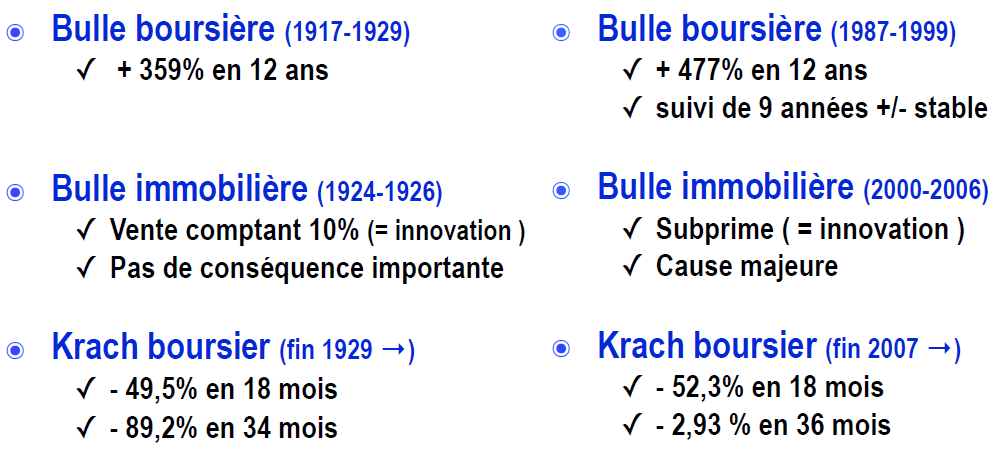
\includegraphics[scale=0.3]{43}
\end{wrapfigure}
\noindent On va établir ici les similitudes et les différences qui existent entre les crises de 1929 et de 2008. Le slide repris ci-contre est assez explicite. La seule chose à rajouter est que la première bulle immobilière (à gauche) concerne juste la Floride alors que la deuxième (à droite) concerne tout le pays ! 
\\\\
Les deux graphiques repris ci-dessous, représente le \textbf{Dow jones Industrial} (définition sur le graphique) pour des périodes reprenant les deux crises. \\
On peut voir sur le premier que l'économie ne se porte pas très mal entre 1946 et 2006, malgré une chute vers 2000. On voit que la bourse explose en raison des grosses spéculations de cette époque. \\
Sur le deuxième graphique, on reprend la période entre 1896 et 1936 (pour la crise de 29). On peut voir qu'à cette époque, la valeur de l'action n'est pas stable mais qu'à partir de 1925 on investit dans l'immobilier et donc on gagne bien. C'est là qu'à partir du 3 septembre 1929, on a le krach ! \\

\begin{minipage}{0.5\textwidth}
	\begin{flushleft}
		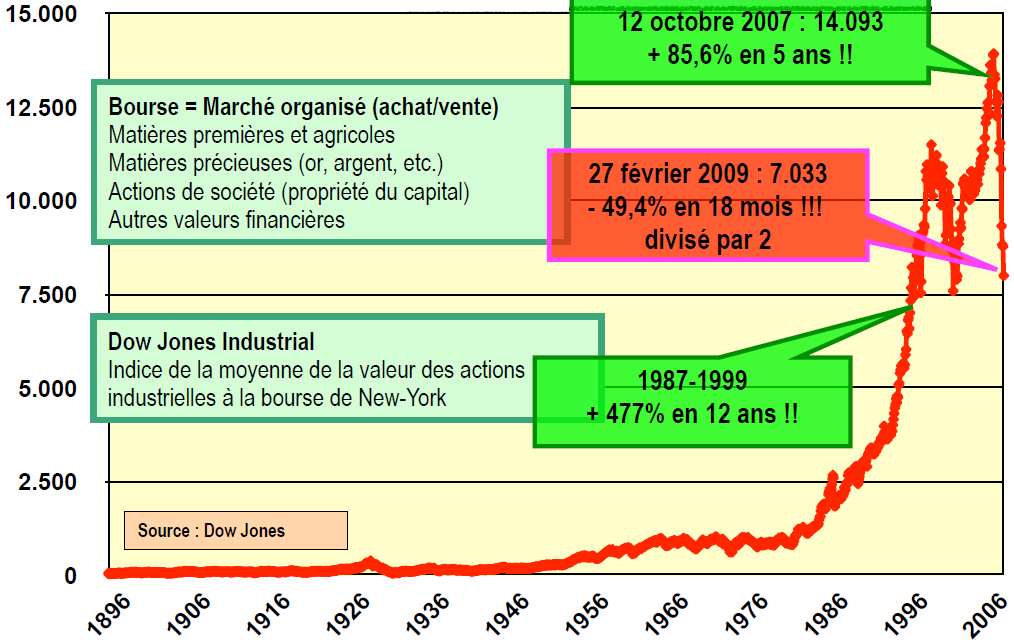
\includegraphics[scale=0.26]{44}
	\end{flushleft}
\end{minipage}
\begin{minipage}{0.5\textwidth}
	\begin{center}
		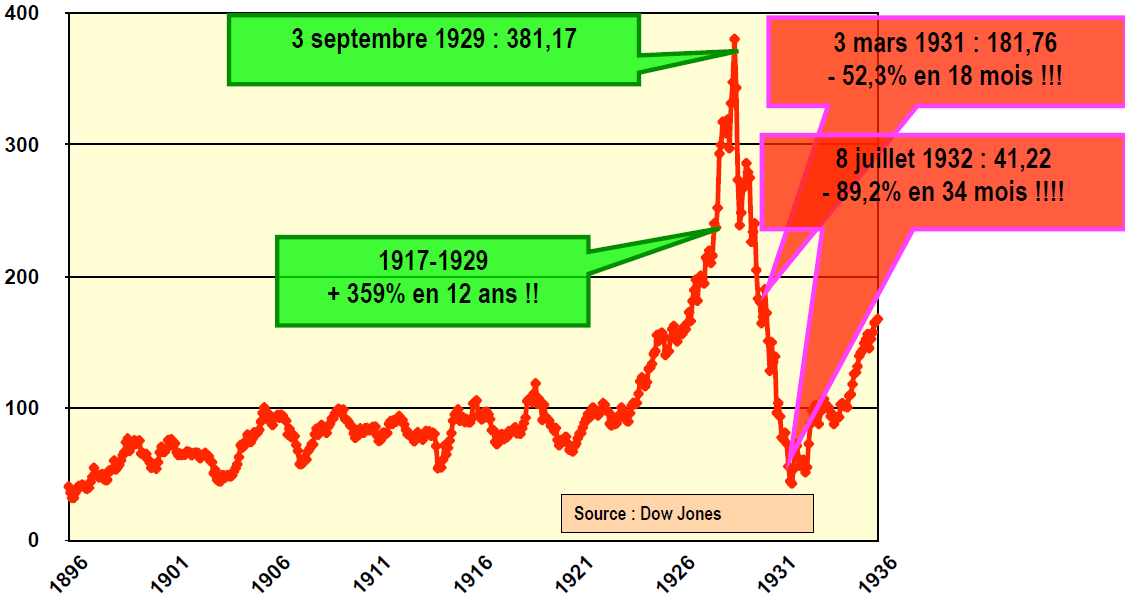
\includegraphics[scale=0.29]{45}
	\end{center}
\end{minipage}
\\
\begin{wrapfigure}[8]{l}{8.5cm}
	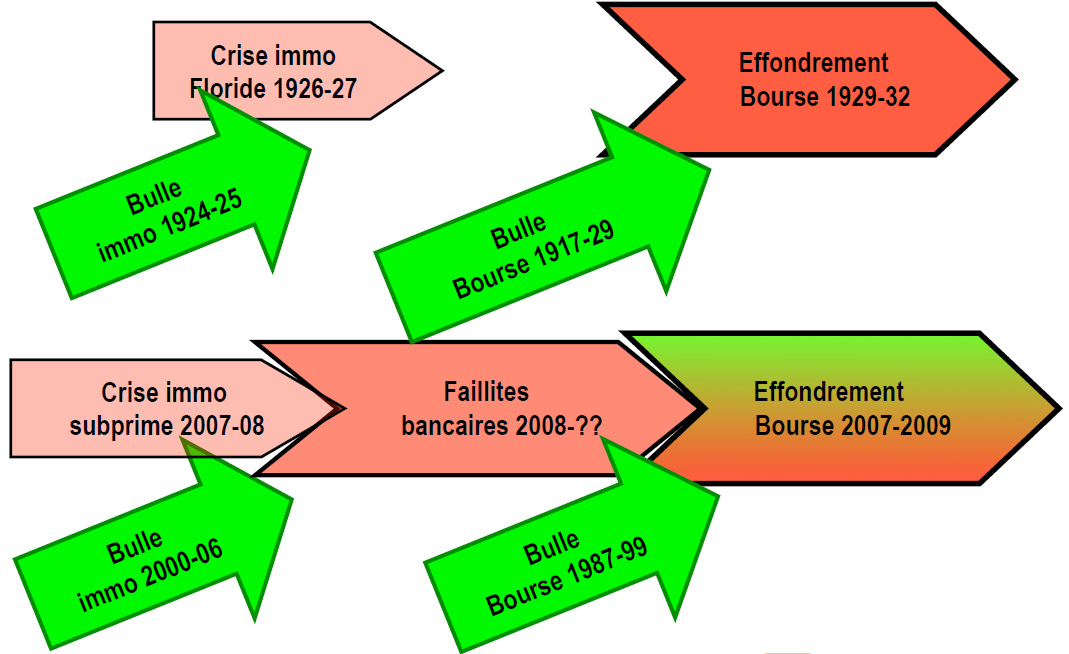
\includegraphics[scale=0.3]{46}
\end{wrapfigure}
\ \\ On peut cependant remarquer la grande similitude qu'il y a entre ces deux crises. En effet, on a toujours cette bulle économique avant l'effondrement. C'est ceci qui est illustré sur le graphique ci-contre. \\\\\\\\\\

\subsection{Innovations financières en 1929}
Tout d'abord, l'Europe avait besoin de réinvestir après la guerre donc il fallait des facilités. Les banques centrales d'Allemagne, France et UK demande a la Federal Reserve d'abaisser sont taux d'intérêt. Celui baisse le taux d'escompte\footnote{Taux d'intérêt auxquel la Federal Reserve prête aux banques.} à 3.5\%. Les banques ont donc accès facilement à l'argent et donc on peut prêter pour investir en bourse. \\
On a ensuite une innovation boursière, l'\textbf{achat d'actions sur marge}, qui consiste à effectuer des ventes inconditionnelles (pas compris, mail envoyé à Alle, attente de réponse) et de pratiquer l'effet de levier comme nous le connaissons dans les années 2000. \\
Ceci a eu pour conséquence l'esplosion des montants prêtés, mais aussi des taux (ils passent de 5\% à 12\% en 1928). Les banquiers font donc la fête (wouhou). 

\subsection{Bulle boursière}
Mais est-ce que c'est en raison de la croissance de l'économie qu'on a la bulle boursière ? Il faut savoir que la valeur des actions est le reflet des profits générés. En effet :

\begin{itemize}
	\item Si les profits croissent $\rightarrow$ dividendes payées $\rightarrow$ \textbf{hausse de la bourse}
	      	
	\item Si les perspectives de profit $\nearrow$ $\rightarrow$ anticipation de l'évolution $\rightarrow$ \textbf{hausse de la bourse}
\end{itemize}

Il est clair que si c'est le contreaire qui se passe, ça entraîne la baisse de la bourse. Pour mesurer les hausses justifié (si une action est rentable), on effectue le rapport cours de bourse / bénéfice (Price Earning Ratio). Ce dernier doit rester raisonable (moyenne entre 1881 et 2008 = 17). L'évolution de ce ratio est repris dans les deux graphiques qui suivent. Les étapes importantes sont indiquées dessus mais on peut dire que l'histoire se répète. \\

\begin{minipage}{0.5\textwidth}
	\begin{flushleft}
		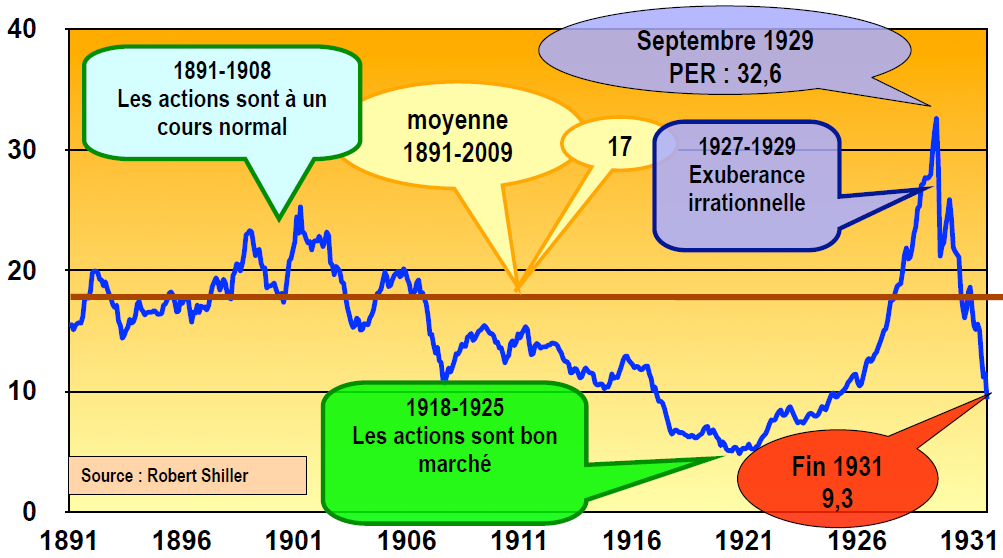
\includegraphics[scale=0.3]{47}
	\end{flushleft}
\end{minipage}
\begin{minipage}{0.5\textwidth}
	\begin{center}
		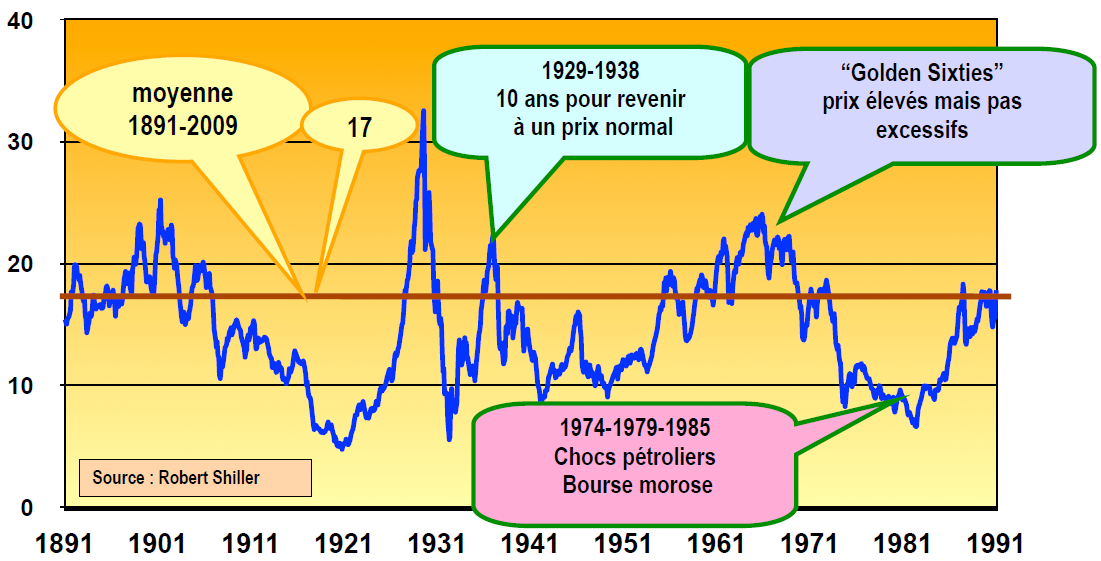
\includegraphics[scale=0.3]{48}
	\end{center}
\end{minipage}

\section{La crise de 1929}

\subsection{Cause}
Certaines grandes banques sont très créatives. Elles prêtent peu aux spéculateurs et créent des structures spéciales pour attirer leur argent. Elles ont aussi des structures de Trust d'investissement qui sont en fait des société spécialisé qui achètent des actions (en pratiquant l'effet de levier), ce sont les précurseurs des fonds actuels. Ces trusts d'investissement explose ! Leur nombre passe de 186 à 265 de 1928 à 1929.
\\\\
Cependant, certains d'entre eux prêtent aux spéculateurs. Du coup, quand la crise est arrivée, les spéculateurs ont perdu beaucoup. Il ne peuvent donc pas rembourser les banques qui perdent à leur tour. De plus, les épargnants perdent confiance et ça entraîne la faillite bancaire. Cependant, contrairement à aujourd'hui, l'Etat n'est pas intervenu. Donc, en même temps que les spéculateurs, les épargnant aussi ont tout perdu.

\subsection{Conséquences}
Ca a eu des conséquences mondiales puisque le commerce international a chuté en volume de -25\% entre 1929 et 1933 et -69\% en valeur (effondrement des prix) ! Ca a également comme conséquence direct, le chômage (12.8 millions de chômeurs aux USA en 1933, 6 en Allemagne et 4 en UK). Tout ceci a évidemment de lourdes conséquences sur le PIB des pays (graphique du PIB américain juste en bas). La deuxième figure est une comparaison entre les deux crises. On peut voir que les réactions ont été totalement différentes puisqu'en 1929 on a laissé la finance partir. Les conséquences sont donc beaucoup plus désastreuses pour 1929 puisque l'économie ne s'est pas remis pendant des années. Même les économistes de la Harvard Economic Society n'ont pas su voir clair. Il publiait tout le temps une remontée de l'économie entre 1929-30. \\

\begin{minipage}{0.5\textwidth}
	\begin{flushleft}
		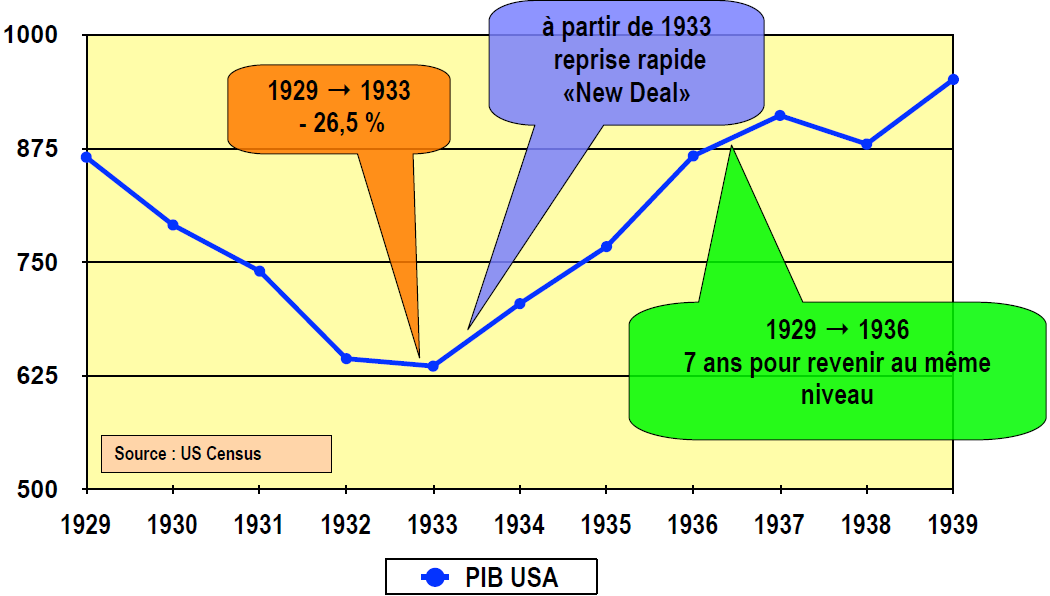
\includegraphics[scale=0.3]{49}
	\end{flushleft}
\end{minipage}
\begin{minipage}{0.5\textwidth}
	\begin{center}
		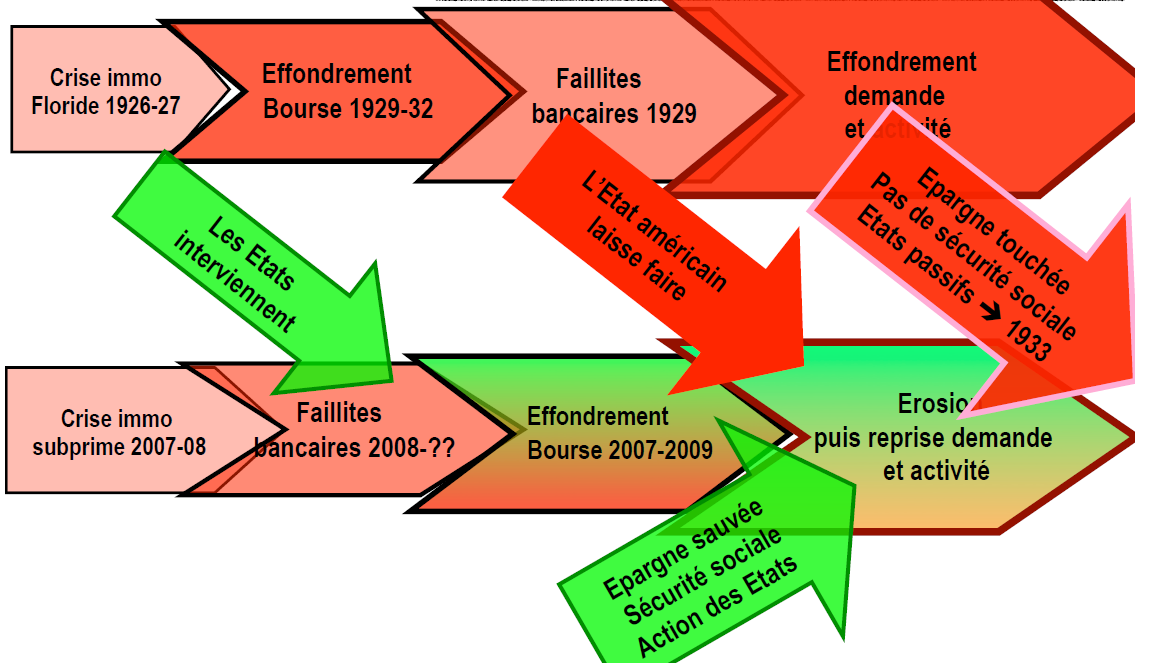
\includegraphics[scale=0.26]{50}
	\end{center}
\end{minipage}

\ \\

Pour finir, voilà la comparaison finale qu'on peut faire entre les deux crises. 

\begin{center}
	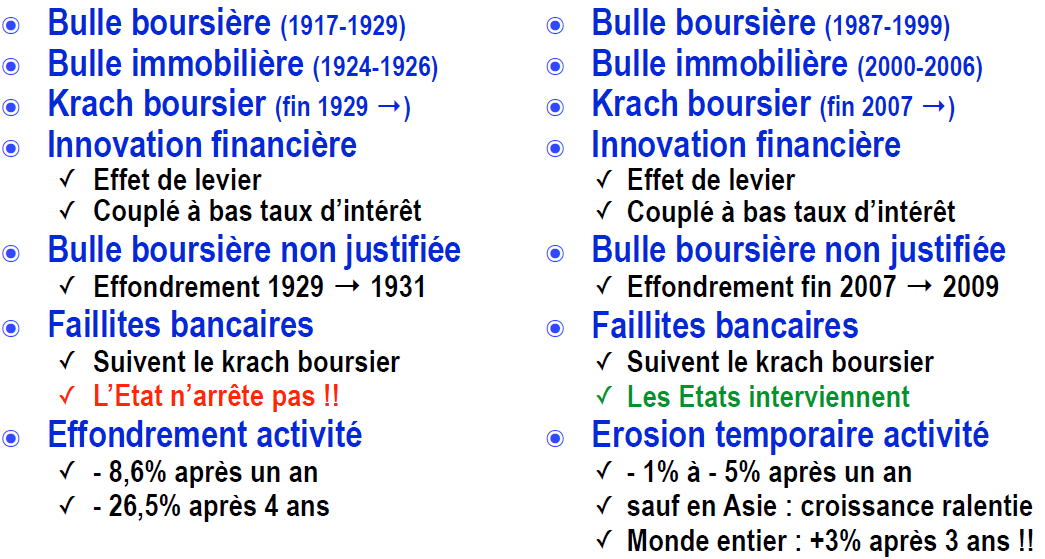
\includegraphics[scale=0.5]{51}
\end{center}

\section{Le rôle de la politique}
\subsection{Etat des lieux}
Différents hommes politiques ont joué de grands rôles en 1933. Parmi ceux-ci, on a F.D.Roosevelt, président américain entre 1933 et 1945 et qui a donc hérité de la crise de 1929. Il a permis de relancer l'économie. On a également Lloyd George, premier ministre anglais, qui a fait de même. \\
Si on revient en 1929, on se rappelle que la quasi-totalité des économistes n'a rien vu venir et d'autre ont nié la réalité de la dépression. De plus, à cette époque, on avait pas d'outil de statistique, on avait pas d'expérience de grande crise antérieure et on avait pas de modélisation économique \footnote{Liens entre les grandes données comme entre l'investissement et le produit national.}. On était donc penché sur l'économie à petite échelle et non sur l'économie dans son ensemble.

\subsection{Vision des libéraux}
Pour les libéraux, la base de l'économie c'est l'entreprise dont l'objectif doit être de maximiser le profit et de minimiser les coûts (notamment le salaire). La pensée était : Profits $\rightarrow$ Investissement $\rightarrow$ Emplois. Pour eux, il faut aussi que le taux d'intérêt suive l'épargne. De cette manière, les entreprises investiront. Cependant, en période de crise, ils ont tendance à diminuer les revenus, donc la consommation et aboutissent à une spirale négative. Donc il faut augmenter les revenus pour augmenter la consommation. 

\subsection{Le marxisme}
Même chose, l'entreprise est la base de l'économie. Ils éxagèrent même au niveau des salaires qui devaient appauvrir les salariés. La crise est bien vu parce que ça rétabli les profits. En effet, le chômage entraîne la baisse des salaires et la faillite d'entreprise fait diminuer la concurrence, donc le profit pour les restants monte. Tout se terminera bien sûr avec une grande crise. 

\section{John Maynard Keynes}
\subsection{Petite biographie}
C'est un homme qui a révolutionné les pensées libérales. Il était professeur à Cambridge et conseiller de l'Etat mais aussi conseiller en investissements financiers. Il s'est fait connaître une première fois au \textbf{Treasury and Peace Conference} pour la discussion des domages de guerre sur l'Allemagne. Il était clairement opposé (l'argent devait rester en Allemagne pour ne pas tuer l'économie). Il a joué un rôle important dans les crises des années '20 et '30. 

\subsection{La crise}
Lui non plus n'a pas vu arriver la crise. Il était très confiant en 1926 mais en 1928 il est très pessimiste quant à la crise. Il pense que la bulle financière américaine n'est pas basé sur la réalité de l'économie et que les prêts pour action (collateral loans) constituent un danger. Cependant, il se trompe en tant qu'investisseur financier \footnote{Son portefeuille financier passe de 44000 à 7815 en 2 ans !} alors qu'il est un très bon conseiller. \\
Mais Keynes perçoit aussi les conditions d'équilibre de l'économie. Les trucs importants sont : 

\begin{itemize}
	\item \textbf{La demande globale}
	\item \textbf{L'anticipation des entrepreneurs} sur la décision investir et donc, sur la demande globale 
	\item \textbf{L'anticipation des consommateurs} sur la décision d'épargner, donc de consommer et sur la demande globale. 
	\item \textbf{Du taux d'intérêt} sur la décision d'investir 
\end{itemize} 

\subsection{Modèle simple de l'économie}
\begin{wrapfigure}[7]{l}{9 cm}
	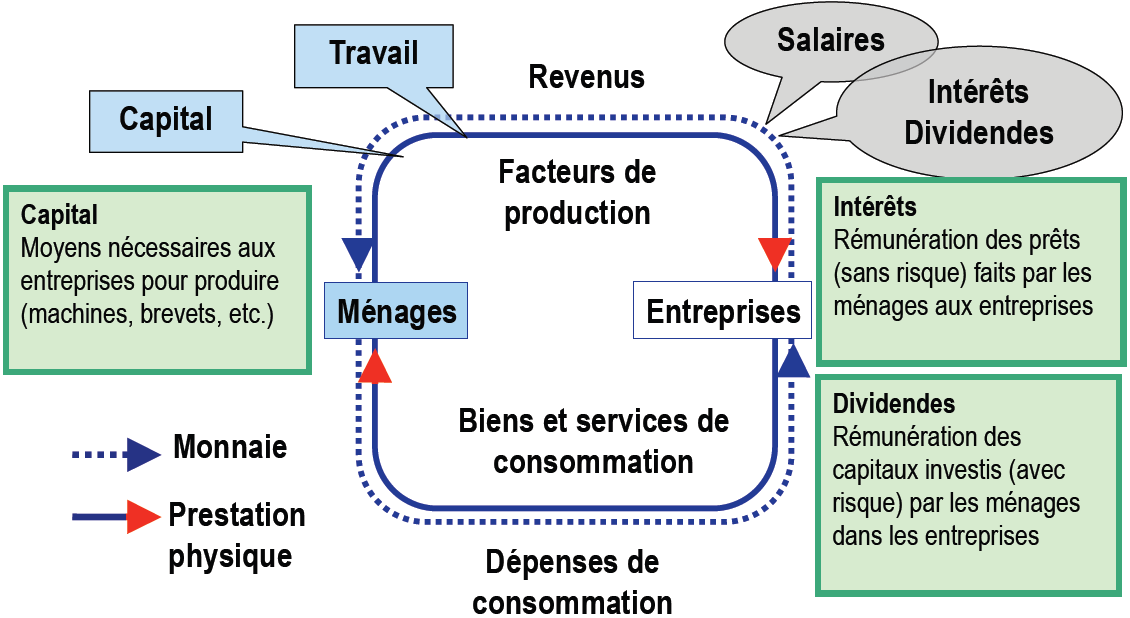
\includegraphics[scale=0.3]{52}
\end{wrapfigure}
De cela découle différents modèles de l'économie dont celui-ci. On a une boucle fermé qui montre que les ménages et les entreprises sont fortement liés. Le schéma est bien représentatif et aucune information supplémentaire n'est nécessaire. \\\\

\begin{wrapfigure}[5]{l}{9 cm}
	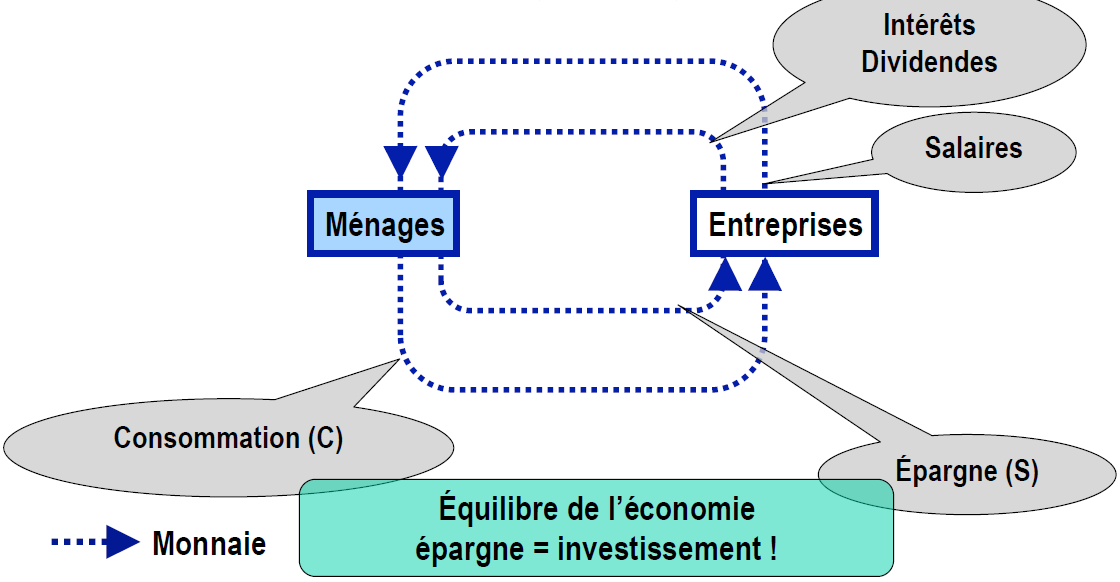
\includegraphics[scale=0.3]{53}
\end{wrapfigure}
On peut voir plus clairement sur ce schéma là que l'équilibre de l'économie serait permise si la totalité de l'épargne était investit en entreprises. Ce n'est bien sûr pas très réaliste.  \\\\\\\\\\\

\section{Modèle réaliste de l'économie}
\begin{wrapfigure}[9]{l}{9 cm}
	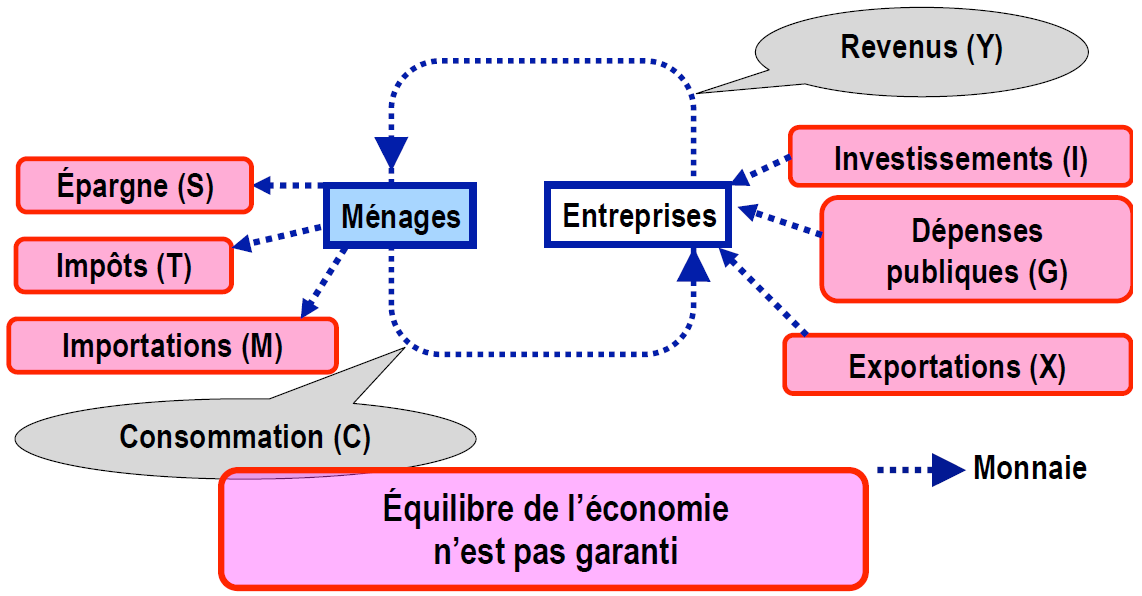
\includegraphics[scale=0.3]{54}
\end{wrapfigure}
Un modèle réaliste serait celui-ci puisque toutes les fuites et injections sont représentées. On a donc en plus du côté ménage les impôts et les importations et du coté entreprise on a que du bon, les investissements (les banques prêtent aux entreprises), les dépenses publiques (injectées par l'Etat) et les exportations. \\\\

\subsection{Consommation et épargne}
Penchons-nous d'un peu plus près sur ces deux termes. Le \textbf{revenu ($Y_d$)} des ménages consiste en le revenu du travail (salaires, ...), revenu du capital (actions, ...), les transferts (allocations familiales, chômage, ...) \textbf{mais} il faut retirer de cela le impots. \\
Le consommateur va partagerr son revenu en \textbf{consommation ($C$)} et \textbf{épargne ($S$)} : 
\begin{equation}
	Y_d = C + S
\end{equation}

Généralement, plus on gagne, plus la part de l'épargne augmente. On introduit donc la propension (part) moyenne du revenu consacré à la \textbf{consommation} comme étant $C/Y_d$ et celle consacré à \textbf{l'épargne} comme étant $S/Y_d$. \\
On va aussi introduire la \textbf{propension marginale} à consommer et à épargner (si on touche un euro en plus qu'est ce qu'on en fait) comme respectivement $\Delta C/\Delta Y_d$ et $\Delta S/\Delta Y_d$.

\subsection{Lien entre consommation et revenue}
On a observé empiriquement que la consommation évoluait linéairement avec le revenu. On a donc, avec des constantes $a$ et $b$ :

\begin{equation}
	C = a + b \cdot Y_d 
\end{equation}

La \textbf{propension marginale à consommer} (variation de la consommation) est donné par $C' = b$. La \textbf{propension moyenne à consommer} est alors donné par 

\begin{equation}
	\frac{C}{Y_d} = \frac{a}{Y_d} + b
\end{equation}

En remplaçant C par sa nouvelle expression

\begin{equation}
	S = Y_d - C = Y_d(1-b) + a
\end{equation}

Pour faire le compte des entreprises, on a comme entré d'argent la consommation, l'investissement (I), les dépenses publiques (G) et les exportations (X) et en argent perdu il y a les importations (M) : 

\begin{equation}
	AD = C + I + G + X - M
\end{equation}

Pour faire évoluer la demande globale, on peut agir sur chaque composante. On cherche donc une relance en cas de dépresson et un ralentissement en cas de surchauffe. \\
Le plus facile est d'agir sur les \textbf{investissements} car ce sont des décisions directes pour le public et il suffit de faire varier les taux d'intérêt au niveau privé. \\
On peut également jouer sur la consommation en réduisant les impôts et en ajoutant des allocations spécifiques. 

\begin{wrapfigure}[11]{l}{9 cm}
	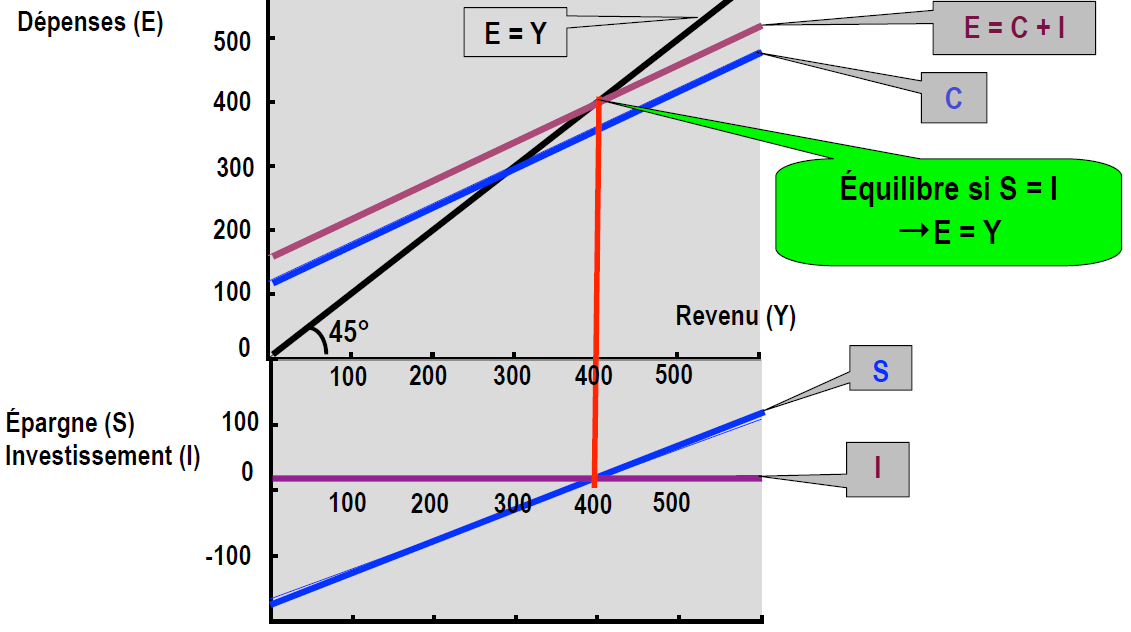
\includegraphics[scale=0.3]{55}
\end{wrapfigure}
On aboutit au graphique ci-contre qui représente en bas, le ménage et en haut l'entreprise. On considère que le ménage consomme et investit et donc que son épargne augmente encore plus avec le revenu. On considère également que l'entreprise dépense ce qu'il gagne. On remarque que l'intersection entre \textbf{l'équilibre} et la courbe E est atteinte lorsque $S = I$. Il faudrait donc que \textbf{l'épargne soit totalement investit}. 

\subsection{Rôle de la confiance}
\begin{wrapfigure}[9]{l}{9 cm}
	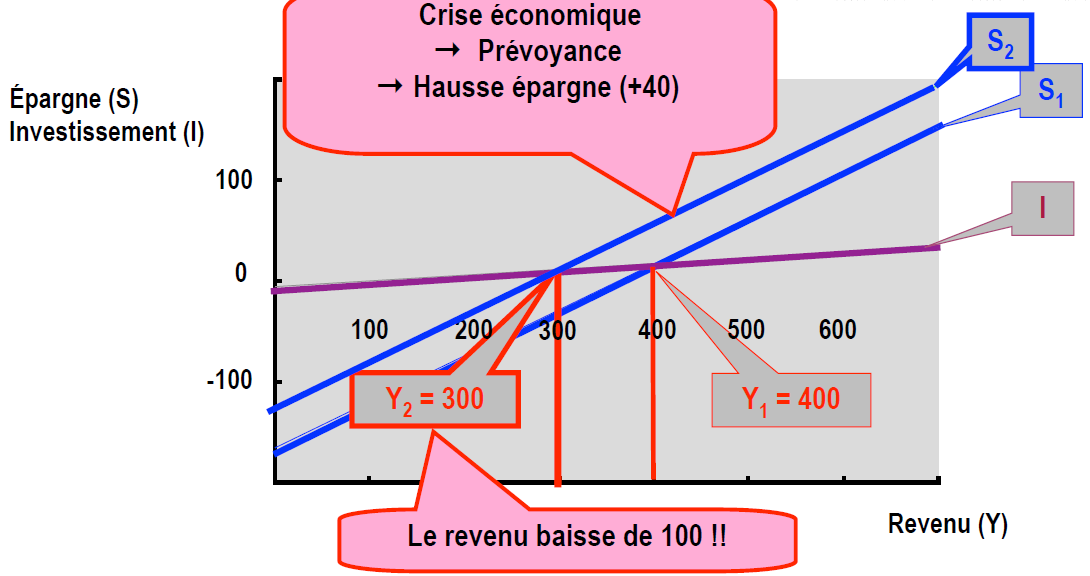
\includegraphics[scale=0.3]{56}
\end{wrapfigure}
Nous sommes maintenant en plein \textbf{paradoxe de la prévoyance}. Mettons-nous dans le cas où c'est la crise économique et que tout le monde augmente sont épargne par prévoyance. Ceci entraîne la remontée de la courbe et on voit qu'on croise la courbe des revenus à 300 et plus à 400. Le revenu a donc baissé de 100 ! \\

\section{Multiplicateur de l'investissement}
C'est la découverte majeure de Keyne. Le principe est qu'en injectant de l'investissement dans l'économie, on va créer du revenu supplémentaire. Intuitivement, \\
$
\mbox{Plus d'investissement} \rightarrow \mbox{plus de production} \rightarrow  \mbox{plus d'emploi} \rightarrow \mbox{plus de revenu} \rightarrow \mbox{plus de consommation} \\ \rightarrow \mbox{confiance en l'avenir} \rightarrow \mbox{les entreprises investissent} \rightarrow \mbox{cercle vertueux !}
$ \\
On peut aussi voir que sur le dernier graphique, si on fait monter la barre I, le revenu augmente. \\
Il persiste néanmoins un problème car le risque de fuite est élevé. En effet, si un Etat relance seul son économie par l'investissement public, on achètera à l'étranger, ce qui augmente les importations et on perd une partie importante du multiplicateur. Pour résoudre ce problème, on ferme les frontières aux importations. Cependant, si les autres pays ferment également leurs frontières, il y aura moins de concurrence et donc les prix monteront. 

\section{Le "New Deal"}
L'objectif de ce "nouvel accord" est de sortir de la grande dépression. Pour cela, il fallait \textbf{soutenir les plus pauvres} (assitance sociale, aides par le travail, Social Security System), \textbf{réformer les marchés financiers} (contrôle bourse et banques) et \textbf{relancer la demande globale} (investissement, consmmation des plus pauvres). \\
On a également \textbf{lutter contre le chômage} en payant des indemnités de chômage et en remettant les chômeurs les plus jeunes au travail, fait \textbf{des grands travaux} (électrification, routes), crée un système de \textbf{protection sociale} notamment la retraite et on a introduit des \textbf{libertés syndicales}. \\
Le résultat est \textbf{40 ans de stabilité et de croissance économique}. On termine le chapitre avec un résumé des idées de Keynes ci-bas. \\

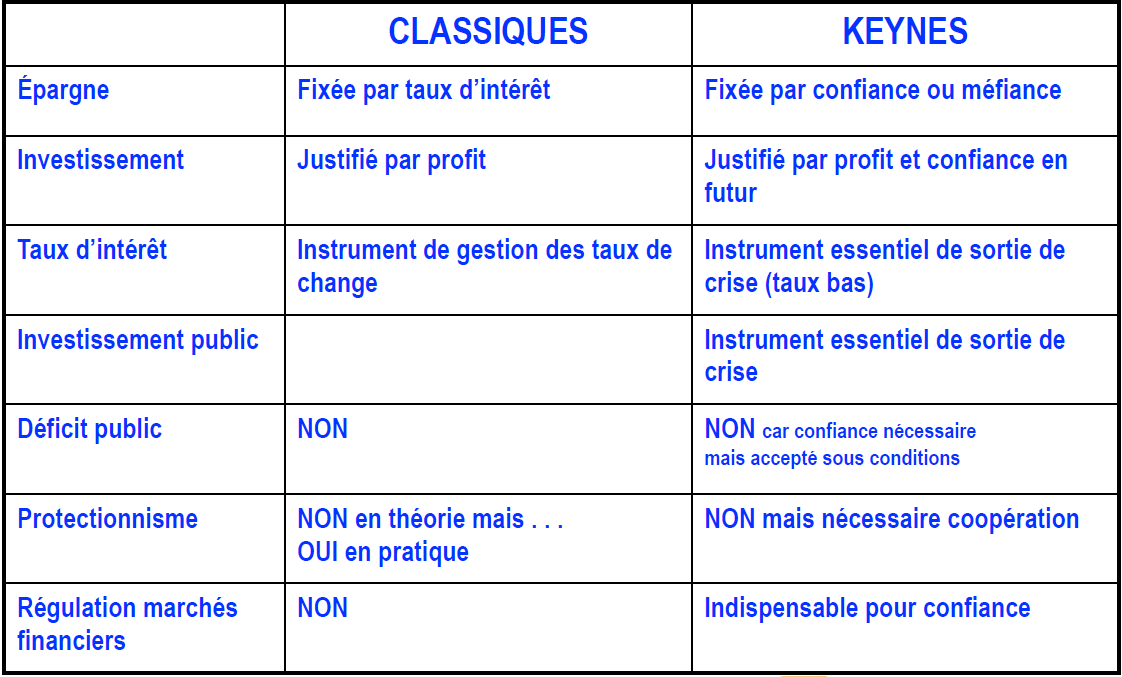
\includegraphics[scale=0.5]{57}